%%%%%%%%%%%%%%%%%%%%%%%%%%%%%%%%%%%%%%%%%%%%%%%%%%%%%%%%%%%%%%%%%%%%
%% I, the copyright holder of this work, release this work into the
%% public domain. This applies worldwide. In some countries this may
%% not be legally possible; if so: I grant anyone the right to use
%% this work for any purpose, without any conditions, unless such
%% conditions are required by law.
%%%%%%%%%%%%%%%%%%%%%%%%%%%%%%%%%%%%%%%%%%%%%%%%%%%%%%%%%%%%%%%%%%%%

\documentclass[
  digital,     %% The `digital` option enables the default options for the
               %% digital version of a document. Replace with `printed`
               %% to enable the default options for the printed version
               %% of a document.
%%  color,       %% Uncomment these lines (by removing the %% at the
%%               %% beginning) to use color in the printed version of your
%%               %% document
  oneside,     %% The `oneside` option enables one-sided typesetting,
               %% which is preferred if you are only going to submit a
               %% digital version of your thesis. Replace with `twoside`
               %% for double-sided typesetting if you are planning to
               %% also print your thesis. For double-sided typesetting,
               %% use at least 120 g/m² paper to prevent show-through.
  nosansbold,  %% The `nosansbold` option prevents the use of the
               %% sans-serif type face for bold text. Replace with
               %% `sansbold` to use sans-serif type face for bold text.
  nocolorbold, %% The `nocolorbold` option disables the usage of the
               %% blue color for bold text, instead using black. Replace
               %% with `colorbold` to use blue for bold text.
  nolof,         %% The `lof` option prints the List of Figures. Replace
               %% with `nolof` to hide the List of Figures.
  nolot,         %% The `lot` option prints the List of Tables. Replace
               %% with `nolot` to hide the List of Tables.
]{fithesis4}
%% The following section sets up the locales used in the thesis.
\usepackage[resetfonts]{cmap} %% We need to load the T2A font encoding
\usepackage[T1,T2A]{fontenc}  %% to use the Cyrillic fonts with Russian texts.
\usepackage[
  main=english, %% By using `czech` or `slovak` as the main locale
                %% instead of `english`, you can typeset the thesis
                %% in either Czech or Slovak, respectively.
  english, german, russian, czech, slovak %% The additional keys allow
]{babel}        %% foreign texts to be typeset as follows:
%%
%%   \begin{otherlanguage}{german}  ... \end{otherlanguage}
%%   \begin{otherlanguage}{russian} ... \end{otherlanguage}
%%   \begin{otherlanguage}{czech}   ... \end{otherlanguage}
%%   \begin{otherlanguage}{slovak}  ... \end{otherlanguage}
%%
%% For non-Latin scripts, it may be necessary to load additional
%% fonts:
\usepackage{paratype}
\def\textrussian#1{{\usefont{T2A}{PTSerif-TLF}{m}{rm}#1}}
%%
%% The following section sets up the metadata of the thesis.
\thesissetup{
    date        = \the\year/\the\month/\the\day,
    university  = mu,
    faculty     = fi,
    type        = bc,
    department  = Department of Computer Systems and Communications,
    author      = Tomáš Marek,
    gender      = f,
    advisor     = {Ing. Milan Brož, Ph.D.},
    title       = {Improvements of the Randomness Testing Toolkit},
    TeXtitle    = {Improvements of the Randomness Testing Toolkit},
    keywords    = {keyword1, keyword2, ...},
    TeXkeywords = {keyword1, keyword2, \ldots},
    abstract    = {%
      This is the abstract of my thesis, which can

      span multiple paragraphs.
    },
    thanks      = {%
      These are the acknowledgements for my thesis, which can

      span multiple paragraphs.
    },
    bib         = bibliography.bib,
    %% Remove the following line to use the JVS 2018 faculty logo.
    facultyLogo = fithesis-fi,
}
\usepackage{makeidx}      %% The `makeidx` package contains
\makeindex                %% helper commands for index typesetting.
%% These additional packages are used within the document:
\usepackage{paralist} %% Compact list environments
\usepackage{amsmath}  %% Mathematics
\usepackage{amsthm}
\usepackage{amsfonts}
\usepackage{url}      %% Hyperlinks
\usepackage{markdown} %% Lightweight markup
\usepackage{listings} %% Source code highlighting
\lstset{
  basicstyle      = \ttfamily,
  identifierstyle = \color{black},
  keywordstyle    = \color{blue},
  keywordstyle    = {[2]\color{cyan}},
  keywordstyle    = {[3]\color{olive}},
  stringstyle     = \color{teal},
  commentstyle    = \itshape\color{magenta},
  breaklines      = true,
}
\usepackage{floatrow} %% Putting captions above tables
\floatsetup[table]{capposition=top}
\usepackage[babel]{csquotes} %% Context-sensitive quotation marks
\begin{document}
%% The \chapter* command can be used to produce unnumbered chapters:
\chapter*{Introduction}
%% Unlike \chapter, \chapter* does not update the headings and does not
%% enter the chapter to the table of contents. I we want correct
%% headings and a table of contents entry, we must add them manually:
\markright{\textsc{Introduction}}
\addcontentsline{toc}{chapter}{Introduction}

% RANDOMNESS TESTINS - 'theoretical' chapter

\chapter{Randomness testing}
Meeting: notes: < 10 pages, define all terms that are used later\\
maybe mention also irreg length tests\\
to define: null-hypothesis, alpha, p-value, statistic \\
Explanations of principles, ideas, some figures are expected here.\\
Maybe accompanied with example on dice, some stupid RNG\\


The goal of this chapter is to explain the mathematical background of randomness testing for users of the \emph{Randomness Testing Toolkit} and make deeper examination of the results easier for them.

\section{Motivation}
Why do we use these tests, some examples of usage
\\


Randomness testing is a form of empirical statistical testing. During the test a distribution of a data set is tested under the null hypothesis, that the data are random. This means that the data contain no patterns and thus each bit has exactly the same probability of being 1 or 0.

In cryptography, the data are usually acquired from output of various cryptographic primitives, where randomness of the output is required or expected. These are usually (pseudo-)random number generators or ciphers. The randomness testing is then used to assess the quality of the data - whether the data are random, or if the data contain patterns (i.e. are non-random).

Each randomness test detects different set of patterns, therefore more tests are usually applied at the data at the same time. Groups of tests that are applied together are called test batteries. Some groups of test might also search for similar patterns in the data, therefore their results might be correlated. TODO: SOURCE In this case it is recommended to use more than only one group of tests.

\section{Process of testing} \label{chap:rand-process}

At the beginning of statistical testing, the \emph{null hypothesis}  ($H_0$) is set. In the case of randomness testing the null hypothesis states, that the data are \emph{random}. Associated with the null hypothesis is the \emph{alternative hypothesis} ($H_1$), which in this case states that the data are not random. Result of the test is that either we \emph{reject} the null hypothesis (i.e. some pattern in the data was found, the data are not random), or the we \emph{do not reject} the null hypothesis (i.e. no proof of non-randomness was found in the data). 

Another step before we start the test is choosing the \emph{significance level} (often denoted as $\alpha$). The usual values TODO: SOURCE is to choose $\alpha$ = 0.05 or $\alpha$ = 0.01. The lower is the significance level, the more sure we can be when we reject the null hypothesis. 

The next step choosing the statistic (i.e. function) of the data used for testing. This statistic determines which kind of patterns are searched for in the current test.



\section{First level testing}

p-values - explanation - what does it mean, how to get them and how to interpret them\\


\section{Second level testing}

 Motivation why first-level testing is not enough\\
 basic principle how does it work - mentioning uniform distribution of first-level p-values\\


Second level testing is used for a further examination of the data and can yield more information than using a first level testing only. For example when we examine the sequence 
\[\epsilon = 0000 0000 0011 0011 0111 1111 1111\]
it will pass the first level test without raising any raising any suspicions of non-randomness with p-value = TODO. However this sequence clearly contains a pattern and therefore there is a low chance that it was generated by a random source. 

To perform a second-level test, we split the original sequence into $n$ equal length non-overlapping sequences. Then we perform a standard statistical test as described in Section \ref{chap:rand-process} on each of these sequences in separate and collect all of the p-values they generated. These tests are then called first-level tests and their respective p-values are called first-level p-values.
\\
 mention difference between ideal continuous and real discrete\\
 explanations of at least KS-statistic and $\chi^2$-test\\


%AVAILABLE SOLUTIONS

\chapter{Available solutions}


This chapter serves to describe various works and programs this thesis connects to. 

\section{Statistical testing batteries}
More or less deep description of each battery. Should contain information about test parameters/settings.\\
\\
If there are any problems with the battery (e.g. tests which read different amount of data from DieHarder). - Discuss colision with the paper\\
Mention overflow detection\\
how batteries interpret results (first/second level, more statistics)\\
strong and weak things \\

\subsection{Dieharder}
Explain p-samples, name tests with irregular read bytes
\subsection{NIST STS}
Explain stream-size and stream-count

\subsection{Test U01}
List all batteries.
Explain repetitions, --bit -nb -w -r -s, mention repeating tests with different parameters


\section{Testing toolkits}\label{analysis}
JUST COPIED FROM WORK TO ACADEMIC WRITING COURSE, TO BE USED AND CHANGED LATER.



In the previous chapter different randomness testing batteries were described. The typical user, however, uses more than one battery, which means installing and running each testing battery individually. Also it is strongly recommended (sometimes even needed) to set up parameters for each test from the battery individually based on tested file and to run this test manually.

Since this approach is not convenient, Ľubomír Obrátil from Center for Research on Cryptography and Security (CRoCS) at FI MU created the Randomness Testing Toolkit (\emph{RTT}). This toolkit allows users to run and configure three test batteries by a single command.

This work was followed by Patrik Vaverčák from Faculty of Electrical Engineering and Information Technology at Slovak University of Technology. He created newer variant of \emph{RTT} called Randomness Testing Toolkit in Python (\emph{rtt-py}). Compared to \emph{RTT}, it contains two additional test batteries. 

\section{Randomness Testing Toolkit}

\emph{RTT} was created in 2017 and its main idea was to combine \emph{Dieharder}, \emph{NIST STS}\footnote{National Institute of Standards and Technology - Statistical Test Suite} and \emph{Test U01} statistical test batteries into one program. It was written in C++. 

The concept of \emph{RTT} is that it acts only as a unified interface of the batteries. Each test battery is executed by \emph{RTT} as a separate program. The \emph{RTT} then collects the output and processes in into a unified format.~\cite[p.~8]{rtt-obratil}

However some problems in the processing of the output were found; these are addressed in chapter \ref{improvements}.

\subsection{Settings}\label{rtt-settings} 
The \emph{RTT} needs to be set up by the user before running. The first part of user settings contains general settings made for the \emph{RTT}, the second part contains configuration for individual test batteries. Each of these parts is stored in its own JSON\footnote{JavaScript Object Notation} file. The original setup description is from

The general settings are stored in \emph{rtt-settings.json} file, which has to be located in the working directory of the \emph{RTT}~\cite[p.~10]{rtt-obratil} . These settings are usually not changed between runs.
The most important setting from the general part are paths to the executable binaries of individual statistical test batteries. This is the only setting that has to be manually filled by the user.

The storage database can also be filled in by the user, but this functionality is often unused. The following general settings have implicit values and do no need to be changed unless the user wishes to. They are paths to storage directories for results and logs of individual runs and execution options (test timeout and maximal number of parallel executions of tests). 

 The battery configurations are dependant on the size of the tested file, therefore the file with the battery configuration is specified for each run of the \emph{RTT}. These configurations are different for each battery (see sections \ref{dieharder}, \ref{nist} and \ref{tu01}), but settings for all of the batteries can be stored together in a single file.~\cite[p.~11]{rtt-obratil}  The \emph{RTT} contains several prepared battery configurations for various sizes of tested file.



\subsection{Output}
The output of \emph{RTT} is in a plain text format. The most important part of the output is the direct report, which is saved in the results directory. At the beginning of the report are general information -- the name of the tested file, the name of the used battery, ratio of passed and failed tests and battery errors and warnings in case there were any.

After the general information is a list of results of individual test runs in a unified format. The fist part of the single test report contains the name of the test and user settings (\emph{e.g. P-sample count in Dieharder battery or Stream size and count in NIST STS battery}). The second part of the single test report are the resulting second-level P-values alongside the names of statistic used (usually Kolmogorov-Smirnov statistic or Chi-Square test). At the end of the single test report is a list of first-level P-values produced by the test. Example of the output can be seen in Figure \ref{fig:rtt_output_example}.

\begin{figure}
  \begin{center}
    %% minimus is about 100 pixels per 1 centimeter or 300 pixels per 1 inch.
    %% The optimum is about 250 pixels per 1 centimeter 
    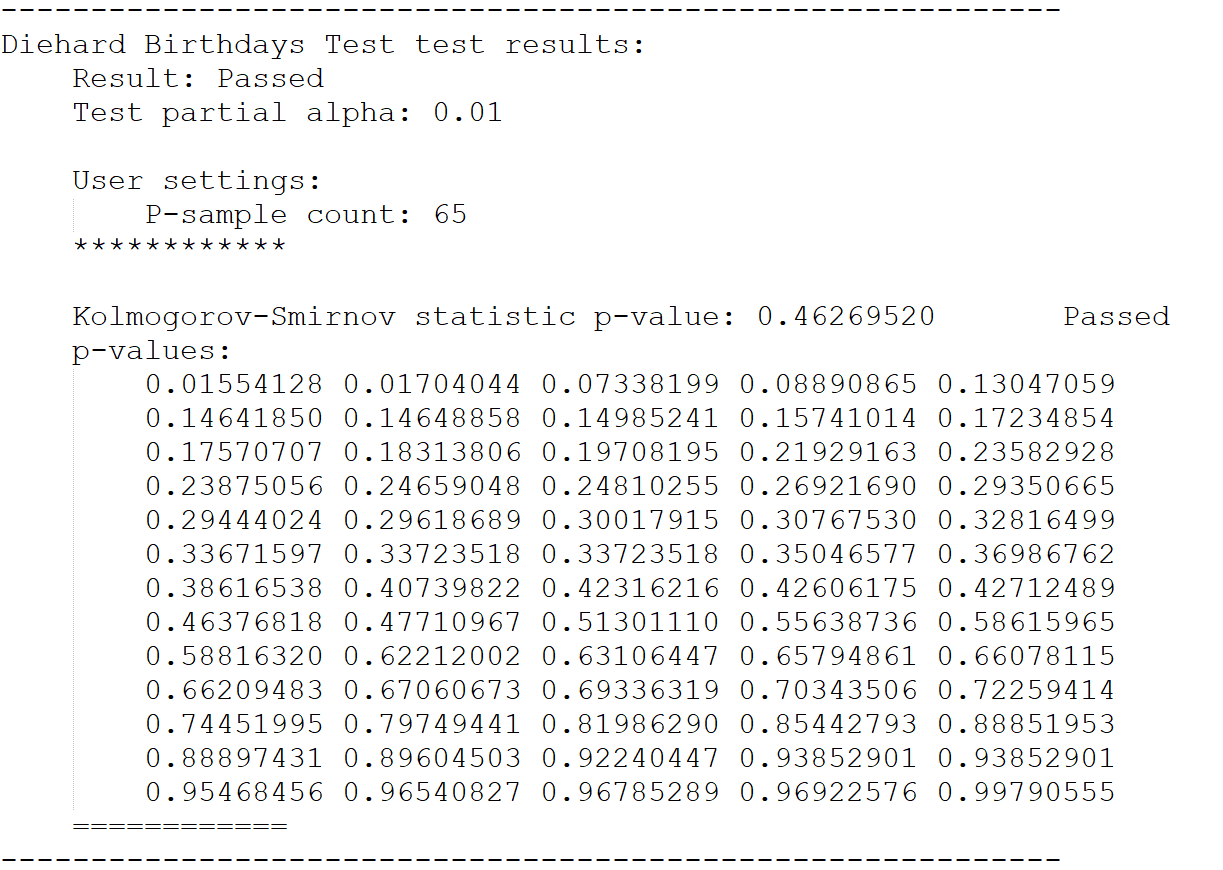
\includegraphics[width=12cm]{figures/rtt_dieharder_output.png}
  \end{center}
  \caption{The example of single test report from the \emph{RTT}}
  \label{fig:rtt_output_example}
\end{figure}

\subsection{Disadvantages}
The problems/weak points we want to improve with this thesis. Namely at least non machine-machine readable format, running only one battery at time, maybe re-calculation of results

There are two most notable disadvantages of the \emph{RTT}. The first one is that each battery has to be run individually by the user. This lowers the convenience of usage for the user. The second one is the output format. While it is easy to read for human users, machine reading requires complicated parsing. 



\section{Randomness Testing Toolking in Python}
The Randomness Testing Toolkit in Python (\emph{rtt-py}) was created by Patrik Vaverčák. It is supposed to be a better version of \emph{RTT}~\cite[p.~24]{vavercak} and it was written in Python. However there are still some functional differences between \emph{RTT} and \emph{rtt-py}. The most notable difference is in the output format and supported batteries.

\subsection{Settings}
The settings of \emph{rtt-py} are very similar to the original \emph{RTT}. According to Vaverčák, the general settings from the \emph{RTT} should be compatible with \emph{rtt-py}, but in reality there is problem with settings for the NIST STS's experiments directory. Also, no database connection is implemented in \emph{rtt-py}, therefore the \emph{mysql-db} attribute is ignored. \cite{rtt-py-github2}


The second part of user settings are tests configurations. They use exactly the same format as those used in \emph{RTT} (as mentioned in \ref{rtt-settings}) and are interchangeable.~\cite[p.~25]{vavercak} The user has to keep in mind that the \emph{rtt-py} uses FIPS\footnote{Federal Information Processing Standards} and BSI\footnote{Bundesamt für Sicherheit in der Informationstechnik} batteries, which are not used in \emph{RTT}.

\subsection{Output}
There is a significant difference in the output format between \emph{RTT} and \emph{rtt-py}. The \emph{rtt-py} creates output in two formats -- \emph{CSV}\footnote{Comma-separated values} and \emph{HTML}\footnote{Hypertext Markup Language}. Both of these report formats contain overview table. Each row from the table represents results of one particular test. The first column contains the name of the test and the name of the battery it belongs to.

The second column contains \emph{failure rate} - ratio representing how many instances of this particular test failed compared to number of executed instances on \emph{all} files with data.


Each of the following columns is named after one tested file. The record contains either P-value reported by the test, or number of failed runs -- this depends on the battery. Example of this table can be seen at figure \ref{fig:rtt_py_table}.
\begin{figure}
  \begin{center}
    %% minimus is about 100 pixels per 1 centimeter or 300 pixels per 1 inch.
    %% The optimum is about 250 pixels per 1 centimeter 
    \frame{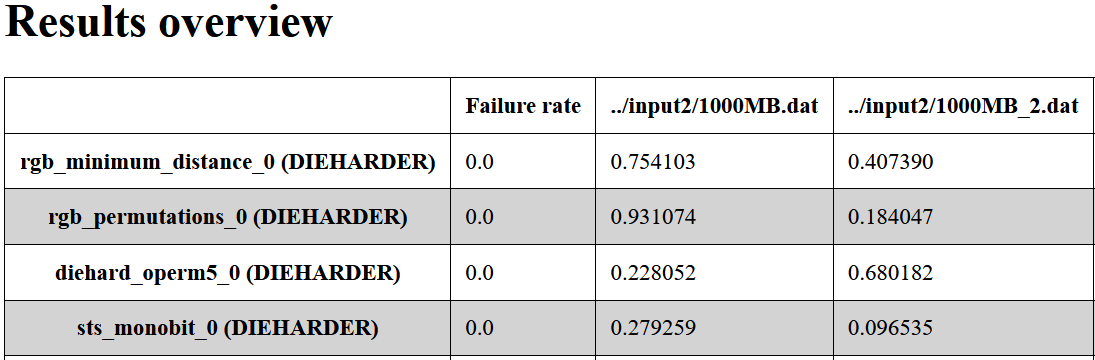
\includegraphics[width=14cm]{figures/rtt-py-table2.png}}
  \end{center}
  \caption{The example of the overview table from the \emph{rtt-py}}
  \label{fig:rtt_py_table}
\end{figure}


The output in the HTML format contains more information compared to the output in the CSV format. For each battery and for each tested file an HTML file with reports is generated.


In each report file there is a list of reports for each executed test from the given battery. The single test report contains the result of the test (either reported P-value, or number of failed runs) and it may contain additional information such as settings of the test or other information connected to the result. The contained information depends on the battery and on the executed test. Example of the  report can be seen in figure \ref{fig:rtt_py_html}
\begin{figure}
  \begin{center}
    %% minimus is about 100 pixels per 1 centimeter or 300 pixels per 1 inch.
    %% The optimum is about 250 pixels per 1 centimeter 
    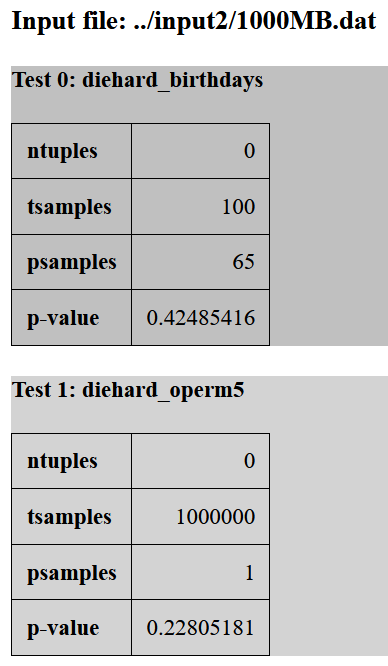
\includegraphics[width=6cm]{figures/rtt-py-dieharder-html.png}
  \end{center}
  \caption{The example of HTML Dieharder report from the \emph{rtt-py}}
  \label{fig:rtt_py_html}
\end{figure}

\subsection{Disdvantages}
One of the problems that need to be addressed is that the \emph{rtt-py } ignores errors and warnings from tests. The most notable example why this is a problem is when the tested file does not contain enough data for current battery configuration.

In this case, the test will read some parts of the data more than once and inform the user about this situation on the error output. The test will still produce result, which will, however, be biased by repeated parts of the tested file.

This may lead to incorrect interpretation of the results and to false acceptance or false rejection of the tested data. Since the \emph{rtt-py} ignores this, there is no way for the user to be informed about this situation.

Compared to the \emph{RTT} the reports created by \emph{rtt-py} contain less information. Namely the first-level P-values are ignored, even though they can be useful for deeper examination of the results and the generator.


% TEST ANALYSIS
\chapter{Tests Analysis}
\section{Data Consumption}
\section{Time Consumption ??}
\section{Configuration Calculator}
goal of the config calc, description, usage etc...
\section{P-Values}
Various problems with test p-values distributions, will probably be split into more sections



% IMPLEMENTATIONS COMPARISON
\chapter{Implementations Comparison}

\section{Output}
Mentioned differences\\
for both RTT and rtt-py - subset or whole?

\section{Missing Features of \emph{rtt-py}}

\section{Proposed improvements}
included things: adding first-level p-values, 

% CONCLUSION

\chapter{Conclusion}






\appendix %% Start the appendices.
\chapter{An appendix}
Here you can insert the appendices of your thesis.

\end{document}
